\documentclass{article}
\usepackage[dvipsnames]{xcolor}
\usepackage[paperwidth=20cm, paperheight=5.5cm, margin = 0cm, top=0.25cm]{geometry}

\usepackage{pgf}
\usepackage{tikz}
\usetikzlibrary{arrows,automata}
\usetikzlibrary{positioning, calc}
\tikzstyle{source}  = 
[
	draw,circle,fill=black,thick,inner sep=0mm,minimum size=2mm
]

\tikzstyle{box}  =
[
	draw,rectangle,thick,inner sep=2mm,
	minimum width=8mm, minimum height=8mm
]

\tikzstyle{redbox} = 
[
	draw,rectangle,thick,inner sep=2mm,
	minimum width=8mm, minimum height=8mm,
	fill=red, opacity=0.3, text opacity=1, draw opacity=1
]

\tikzstyle{dredbox} = 
[
	draw,rectangle,thick,inner sep=2mm,
	minimum width=8mm, minimum height=8mm,
	fill=red, opacity=0.5, text opacity=1, draw opacity=1
]


\tikzstyle{bluebox} = 
[
	draw,rectangle,thick,inner sep=2mm,
	minimum width=8mm, minimum height=8mm,
	fill=blue, opacity=0.3, text opacity=1, draw opacity=1
]

\tikzstyle{greenbox} = 
[
	draw,rectangle,thick,inner sep=2mm,
	minimum width=8mm, minimum height=8mm,
	fill=green, opacity=0.3, text opacity=1, draw opacity=1
]

\tikzstyle{lgreenbox} = 
[
	draw,rectangle,thick,inner sep=2mm,
	minimum width=8mm, minimum height=8mm,
	fill=SpringGreen
]

\tikzstyle{dgreenbox} = 
[
	draw,rectangle,thick,inner sep=2mm,
	minimum width=8mm, minimum height=8mm,
	fill=ForestGreen, opacity=0.5, text opacity=1, draw opacity=1
]


\tikzstyle{bluestate}  = 
[
	state, draw=blue, line width=2pt,
	fill=LimeGreen
]

\tikzstyle{redstate}  = 
[
	state, draw=red, line width=2pt,
	fill=LimeGreen
]

\tikzstyle{violetstate}  = 
[
	state, draw=Violet, line width=2pt,
	fill=LimeGreen
]
 

\begin{document}
\begin{center}
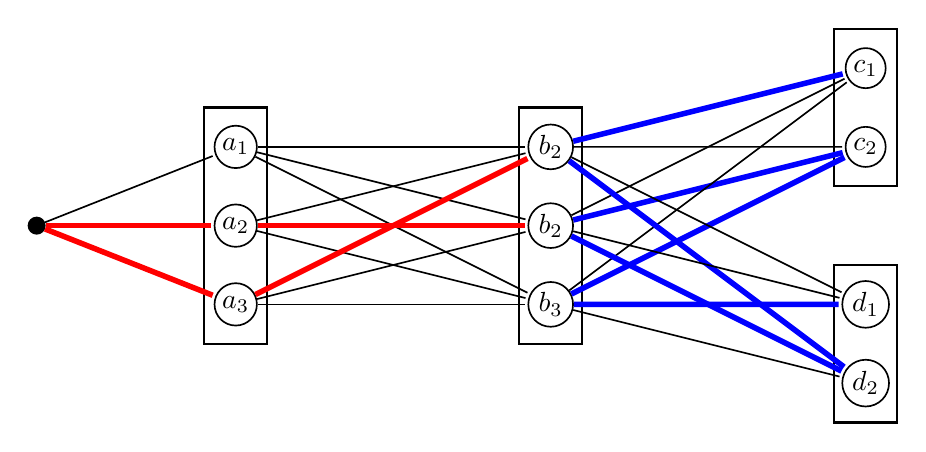
\begin{tikzpicture}[->,>=stealth',shorten >=1pt,auto,node distance=4cm,semithick]

\node[source] (S) {};


\node[box, minimum height=3cm] (A) [right=2cm of S]{};
\node[draw, circle, inner sep=0.5mm] (A2) at (A) {$a_2$};
\node[draw, circle, inner sep=0.5mm] (A1) at ($(A)+(0.0cm, 1.0cm)$) {$a_1$};
\node[draw, circle, inner sep=0.5mm] (A3) at ($(A)+(0.0cm,-1.0cm)$) {$a_3$};

\node[box, minimum height=3cm] (B) [right of = A] {};
\node[draw, circle, inner sep=0.5mm] (B2) at (B) {$b_2$};
\node[draw, circle, inner sep=0.5mm] (B1) at ($(B)+(0.0cm,+1.0cm)$){$b_2$};
\node[draw, circle, inner sep=0.5mm] (B3) at ($(B)+(0.0cm,-1.0cm)$){$b_3$};

\node[box, minimum height=2cm] (C) [right of = B, yshift=1.5cm] {};
\node[draw, circle, inner sep=0.5mm] (C1) at ($(C)+(0.0cm,+0.5cm)$) {$c_1$};
\node[draw, circle, inner sep=0.5mm] (C2) at ($(C)+(0.0cm,-0.5cm)$) {$c_2$};

\node[box, minimum height=2cm] (D) [right of = B, yshift=-1.5cm] {};
\node[draw, circle, inner sep=0.5mm] (D1) at ($(D)+(0.0cm,+0.5cm)$) {$d_1$};
\node[draw, circle, inner sep=0.5mm] (D2) at ($(D)+(0.0cm,-0.5cm)$) {$d_2$};


\path
	(S) edge[-] (A1)
	(S) edge[-,red, line width=2pt] (A2)
	(S) edge[-,red, line width=2pt] (A3);


\path
	(A1) edge[-] (B1)
	(A1) edge[-] (B2)
	(A1) edge[-] (B3)
	(A2) edge[-] (B1)
	(A2) edge[-,red, line width=2pt] (B2)
	(A2) edge[-] (B3)
	(A3) edge[-,red, line width=2pt] (B1)
	(A3) edge[-] (B2)
	(A3) edge[-] (B3)
	;

\path
	(B1) edge[-,blue, line width=2pt] (C1)
	(B1) edge[-] (C2)
	(B2) edge[-] (C1)
	(B2) edge[-,blue, line width=2pt] (C2)
	(B3) edge[-] (C1)
	(B3) edge[-,blue, line width=2pt] (C2);
	
\path
	(B1) edge[-] (D1)
	(B1) edge[-, blue, line width=2pt] (D2)
	(B2) edge[-] (D1)
	(B2) edge[-, blue, line width=2pt] (D2)
	(B3) edge[-, blue, line width=2pt] (D1)
	(B3) edge[-] (D2);


\end{tikzpicture}
\end{center}

\end{document}
                    
\node[state, fill=LimeGreen] (X1) {$A$}; 
\node[state, fill=LimeGreen] (X2) [above=1.0cm of X1, xshift=2cm] {$B$};                   
\node[state]                 (X3) [right of=X1] {$D$};
\node[state, fill=LimeGreen] (X4) [below=1.0cm of X1, xshift=2cm] {$C$};                   
\node[state, fill=LimeGreen] (X5) [right of=X2] {$E$};                   
\node[state, fill=LimeGreen] (X6) [right of=X4] {$F$}; 

\node[box][above=0.25cm of X1](E1){$\varepsilon_A$};                  
\node[box][above=0.25cm of X2](E2){$\varepsilon_B$};
\node[box][above=0.25cm of X4](E4){$\varepsilon_C$};                  
\node[box][above=0.25cm of X5](E5){$\varepsilon_E$};                  
\node[box][above=0.25cm of X6](E6){$\varepsilon_F$};                  

\node[lgreenbox][below=0.25cm of X1, xshift=-1cm](P1){$\pi_A,\lambda_A,p_A$};                  
\node[lgreenbox][below=0.25cm of X2, xshift=+1cm](P2){$\pi_B,\lambda_B,p_B$};  
\node[lgreenbox][below=0.25cm of X3, xshift=-1cm](P3){$\pi_D,\lambda_D,p_D$};                  
\node[lgreenbox][below=0.25cm of X4, xshift=+1cm](P4){$\pi_C,\lambda_C,p_C$};                  
\node[lgreenbox][below=0.25cm of X5, xshift=+1cm](P5){$\pi_E,\lambda_E,p_E$};                  
\node[lgreenbox][below=0.25cm of X6, xshift=+1cm](P6){$\pi_F,\lambda_F,p_F$};                  


\path
	(X1) edge (X2)
	(X1) edge (X3)
	(X1) edge (X4)
	(X3) edge (X6)
	(X3) edge (X5);

\path
	(X1) edge[-] (E1)
	(X2) edge[-] (E2)
	(X4) edge[-] (E4)
	(X5) edge[-] (E5)
	(X6) edge[-] (E6);

\path
	(X1) edge[-] (P1)
	(X2) edge[-] (P2)
	(X3) edge[-] (P3)
	(X4) edge[-] (P4)
	(X5) edge[-] (P5)
	(X6) edge[-] (P6);

\end{tikzpicture}
\end{center}

\end{document}
